% 1987 年全国卷理科第 6 题：y=sin 2x 图象
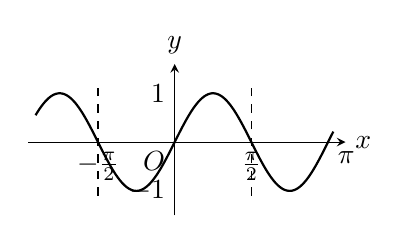
\begin{tikzpicture}[scale=0.62,>=stealth]
  \draw[->] (-3.0,0)--(3.5,0) node[right] {$x$};
  \draw[->] (0,-1.5)--(0,1.6) node[above] {$y$};
  \draw[thick,domain=-2.85:3.25,samples=160]
    plot (\x,{sin(114.592*\x)});
  \draw[dashed] (-1.57,-1.1)--(-1.57,1.1);
  \draw[dashed] (1.57,-1.1)--(1.57,1.1);
  \node[below] at (-1.57,0) {$-\frac\pi2$};
  \node[below] at (1.57,0) {$\frac\pi2$};
  \node[below right] at (3.14,0) {$\pi$};
  \node[left] at (0,1) {$1$};
  \node[left] at (0,-1) {$-1$};
  \node[below left] at (0,0) {$O$};
\end{tikzpicture}
